%===========================================
%\chapter{Décomposer le problème}
\chapter{Module et références}
\index{décomposer le code}
\index{primitif}\index{reference}
%===========================================

\minitoc

%===================
%\section{Motivation}
\section{Décomposer le problème}
%===================

	Jusqu’à présent, les problèmes que nous avons abordés étaient relativement
	petits.  Nous avons pu les résoudre avec un algorithme d’un seul tenant.
	
	Dans la réalité, les problèmes sont plus conséquents et il devient
	nécessaire de les décomposer en sous-problèmes.  On parle d’une
	\emph{approche modulaire}.  Les avantages d’une telle décomposition sont
	multiples.
	
	\begin{itemize}
	\item
		\textbf{Cela permet de libérer l’esprit.}
		L’esprit humain ne peut pas traiter trop d’informations à la fois
		(\emph{surcharge cognitive}).
		Lorsqu’un sous-problème est résolu,
		il peut se libérer l’esprit et attaquer un autre sous-problème.
	\item
		\textbf{On peut réutiliser ce qui a été fait.}
		Si un même sous-problème apparait plusieurs fois
		dans un problème ou à travers plusieurs problèmes,
		il est plus efficace de le résoudre une fois et
		de réutiliser la solution.
	\item
		\textbf{On accroit la lisibilité.} Si,  un algorithme, appelle un autre
		algorithme pour résoudre un sous-problème, le lecteur ou la lectrice
		verra un nom d’algorithme qui peut être plus parlant que les
		instructions qui se cachent derrière, même s’il y en a peu.  Par
		exemple, \pc{dizaine(nb)} est plus parlant que \pc{nb MOD 100 DIV 10}
		pour calculer les dizaines d’un nombre.
	
\end{itemize}

	Parmis les autres avantages, que vous pourrez moins percevoir en début
	d’apprentissage, citons la possibilité de répartir le travail dans une
	équipe.
	
	Un algorithme qui résout une partie de problème
	est parfois appelé \textbf{fonction}\index{fonction}, 
	\textbf{procédure}\index{procédure}, 
	\textbf{méthode}\index{méthode} ou encore
	\textbf{module}\index{module}
	en fonction du langage et du contexte.
	Il y a quelques nuances mais elles importent peu ici.
	
%===================
\section{Exemple}
%===================

	Illustrons l’approche modulaire sur le calcul du maximum de 3 nombres.

	\begin{center}
	\flowalgoddd{a (réel)}{b (réel)}{c (réel)}{max3}{réel}
	\end{center}
	
	Commençons par écrire la solution du problème plus simple~:~
	le maximum de 2 nombres.

	\begin{minipage}{6cm}
		\flowalgodd{a (réel)}{b (réel)}{max2}{réel}
	\end{minipage}
	\quad
	\begin{minipage}{7cm}
		\begin{pseudocode}
		\Algo{max2}{\Par{a}{real}, \Par{b}{real}}{real}
			\Decl{max}{real}
			\If{a > b}
				\Let max \Gets a
			\Else
				\Let max \Gets b
			\EndIf
			\Return max
		\EndAlgo
		\end{pseudocode}
	\end{minipage}
	
	Pour le maximum de 3 nombres, il existe plusieurs approches.  Voyons
	celle-ci~:

	\begin{enumerate}
		\item  Calculer le maximum des deux premiers nombres, soit \pc{maxab}
		\item  Calculer le maximum de \pc{maxab} et du troisième nombre, ce qui donne le résultat.
	\end{enumerate}

	Elle s'illustre comme suit~:
	
	\begin{center}
	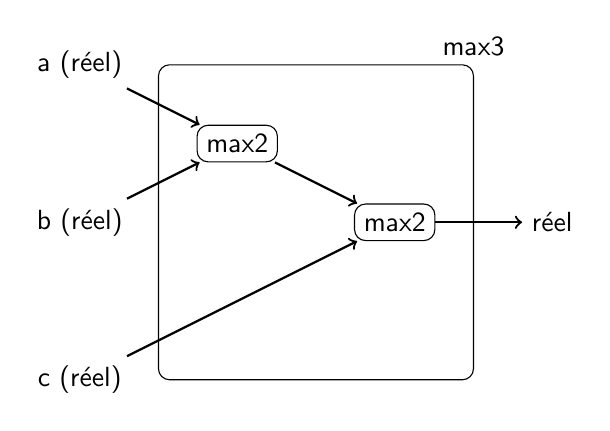
\begin{tikzpicture}[auto]
		\sffamily
		\node (a) at (0,4) {a (réel)};
		\node (b) at (0,2) {b (réel)};
		\node (c) at (0,0) {c (réel)};
		\node[draw,rounded corners] (max2a) at (2,3) {max2};
		\node[draw,rounded corners] (max2b) at (4,2) {max2};
		\node (r) at (6,2) {réel};
		\draw[rounded corners] (1,0) rectangle (5,4) node[above] {max3};
		\draw[->,thick] (a) to (max2a);
		\draw[->,thick] (b) to (max2a);
		\draw[->,thick] (c) to (max2b);
		\draw[->,thick] (max2a) to (max2b);
		\draw[->,thick] (max2b) to (r);
	\end{tikzpicture}	
	\end{center}
	
	Sur base de cette idée, 
	on voit que calculer le maximum de trois nombres
	peut se faire en calculant deux fois le maximum de deux nombres.
	On ne va évidemment pas \emph{recopier}%
	\footnote{
		Cette approche serait fastidieuse,
		engendrerait de nombreuses erreurs lors du recopiage
		et serait difficile à lire. Même le copier/coller n'est pas une bonne 
		solution. Il diminue la lisibilité et rend la refactorisation et 
		l'évolution des alogorithmes et des programmes plus compliquées.
	} dans notre solution
	ce qu’on a écrit pour le maximum de deux nombres~;
	on va plutôt y faire référence, 
	c’est-à-dire appeler l’algorithme \pc{max2}. 
	Ce qui donne~:

	\begin{pseudocode}
	\Algo{max3}{\Par{a}{real}, \Par{b}{real}, \Par{c}{real}}{real}
		\Decl{maxab, max}{reals}
		\Let maxab \Gets max2(a,b)
		\Let max \Gets max2(maxab,c)
		\Return max
	\EndAlgo
	\end{pseudocode}

	qui peut se simplifier en~:
	
	\begin{pseudocode}
	\Algo{max3}{\Par{a,b,c}{reals}}{real}
		\Return max2( max2(a,b) ,c)
	\EndAlgo
	\end{pseudocode}

%===================
\section{Paramètres et valeur de retour}
\index{paramètres}\label{paramètres}
%=======================

	Jusqu’à présent, nous avons considéré que les paramètres d’un algorithme (ou
	\emph{module}\index{module}) correspondent à ses données et que le résultat,
	unique, est retourné.

	Il s’agit d’une situation fréquente mais pas obligatoire que nous pouvons
	généraliser.  En algorithmique nous allons traiter avec trois sortes de 
	paramètres. Nous verrons ensuite que tous les langages n'acceptent pas tous 
	les types de paramètres. 

	%==================================
	\subsection{Le paramètre en entrée}
	\label{param.entrée}
	%==================================

		Le paramètre en \textbf{entrée} est ce que nous connaissons déjà.  Il
		correspond à une donnée de l’algorithme.  Une valeur va lui être
		attribuée en début d’algorithme et elle ne sera pas modifiée.  On pourra
		faire suivre le nom du paramètre d’une flèche vers le bas (\In) pour
		rappeler son rôle mais ce n'est pas obligatoire lorsqu'il n'y a pas
		d'ambiguïté.
		
		Lors de l’appel, c'est une \textbf{valeur} qui est fournie ou, plus
		généralement une expression dont la valeur sera donnée au paramètre.
		Voici un cas général de paramètre en entrée.
		
		\begin{minipage}{4cm}
			\begin{pseudocode}
				\LComment {Code}
				\LComment {appelant}
				\Stmt myAlgo(expr)
				\Empty
			\end{pseudocode}
		\end{minipage}
		\quad
		\begin{minipage}{8cm}
			\begin{pseudocode}
				\LComment {Code appelé}
				\Algo{myAlgo}{\Par{par\In}{integer}}{}
				\Stmt \dots
				\EndAlgo 
			\end{pseudocode}
		\end{minipage}
		
		C’est comme si l’algorithme \pc{myAlgo} commençait par l’affectation
		\pc{par \Gets expr}.
		
		\textbf{Exemple.} 
		Reprenons l’exemple de \pc{max3}
		en ajoutant un petit test.

		\begin{pseudocode}[1]
			\Algo{test}{}{} \RComment {Code appelant}
				\Decl {max}{real}
				\Let max \Gets max3(3, 2, 5)
				\Write max
			\EndAlgo
			\Empty
			\Algo{max3}{\Par{a\In, b\In, c\In}{reals}}{real}
				\RComment {Code appelé}
				\Decl{maxab, max}{reals}
				\Let maxab \Gets max2(a,b)
				\Let max \Gets max2(maxab,c)
				\Return max
			\EndAlgo
		\end{pseudocode}

		Traçons son exécution.
		
		\begin{tabular}{|>{\centering\arraybackslash}m{1.1cm}
						|>{\centering\arraybackslash}m{13mm}
						|*{5}{>{\centering\arraybackslash}m{13mm}}|}
			\hline
			\rowcolor{black!50}
			  & \pc{test} & \multicolumn{5}{c|}{\pc{max3}} \\
			\hline
			\rowcolor{black!30}
			\# & max  & {a} & {b} & {c} & {maxab} & {max}\\
			\hline
			2    & indéfini             &                      &                      &                      &                      &          \\
			3,7  & {\color{gray}$\mid$} & 3                    & 2                    & 5                    &                      &          \\
			8    & {\color{gray}$\mid$} & {\color{gray}$\mid$} & {\color{gray}$\mid$} & {\color{gray}$\mid$} & indéfini             & indéfini \\
			9    & {\color{gray}$\mid$} & {\color{gray}$\mid$} & {\color{gray}$\mid$} & {\color{gray}$\mid$} & 3                    & indéfini \\
			10   & {\color{gray}$\mid$} & {\color{gray}$\mid$} & {\color{gray}$\mid$} & {\color{gray}$\mid$} & {\color{gray}$\mid$} & 5        \\
			11,3 & 5                    &                      &                      &                      &                      &          \\
			\hline
		\end{tabular}
		
		\paragraph{Notez bien~:} Dans cet exemple, on trouve deux fois la
		variable \pc{max}.  Il s’agit bien de deux variables
		\textbf{différentes}~; l’une est définie et connue dans \pc{test}~;
		l’autre l’est dans \pc{max3}.
		
%	%==================================
%	\subsection{Le paramètre en sortie}
%	%==================================
%
%		Le paramètre en \textbf{sortie} correspond à un résultat de
%		l’algorithme.  Avec la notation que nous utilisons, un algorithme ne
%		peut retourner qu’une seule valeur ce qui est parfois une contrainte
%		trop forte.  Les paramètres en sortie vont permettre à l’algorithme de
%		fournir plusieurs réponses.  On fera suivre le nom du paramètre d’une
%		flèche vers le haut (\Out) pour rappeler son rôle.  Un tel paramètre
%		n’aura pas de valeur au début de l’algorithme mais s’en verra attribuer
%		une par l’algorithme.
%		
%		Lors de l’appel, on fournit une \textbf{variable}
%		qui recevra la valeur finale du paramètre.
%		Voici un cas général de paramètre en sortie.
%		
%		\begin{minipage}{4cm}
%			\begin{pc}
%				\LComment {Code appelant}
%				\Stmt myAlgo(variable)
%				\Empty
%			\end{pc}
%		\end{minipage}
%		\quad
%		\begin{minipage}{8cm}
%			\begin{pc}
%				\LComment {Code appelé}
%				\Entete{myAlgo}{\Par{par\Out}{entier}}{}
%				\Stmt \dots
%			\end{pc}
%		\end{minipage}
%
%		Il n’y a \textbf{pas de \pc{\algorithmicreturn}}
%		puisque les résultats sont en paramètres de sortie et pas comme
%		valeur \emph{retournée}.
%		C’est comme si,
%		à la fin de l’algorithme appelé,
%		on avait l’assignation~:
%		\pc{variable \Gets par}.
%		
%		\paragraph{Exemple.}
%		On peut envisager un algorithme
%		qui reçoit une durée exprimée en seconde
%		et fournisse trois paramètres en sortie
%		correspondant à cette même durée exprimée en heures, minutes et secondes.
%		En voici le schéma et la solution~:
%		\begin{center}
%		\flowalgorrr{totalSec (entier)}{versHMS}{heuresÉcoulées (entier)}{minutesÉcoulées (entier)}{secondesÉcoulées (entier)}
%		\end{center}
%			
%		Voici une solution et un appel possible.
%		\begin{pc}[1]
%			\Algo{versHMS}{\Par{totalSec\In, heuresÉcoulées\Out, minutesÉcoulées\Out, secondesÉcoulées\Out}{\\\hfill entiers}}{}
%				\Let heuresÉcoulées \Gets totalSec DIV (60*60)
%				\Let minutesÉcoulées \Gets totalSec MOD (60*60) DIV 60				
%				\Let secondesÉcoulées \Gets totalSec MOD 60
%			\EndAlgo
%			\Empty
%			\Algo{test}{}{}
%				\Decl{heure,minute,seconde}{entiers}
%				\Stmt versHMS(65536, heure, minute, seconde)
%				\Write heure, minute, seconde
%			\EndAlgo
%		\end{pc}
%		
%		Traçons-le.
%
%		\begin{small}
%		\begin{tabular}{|>{\centering\arraybackslash}m{7mm}
%						|*{3}{>{\centering\arraybackslash}m{9mm}}
%						|>{\centering\arraybackslash}m{10mm}
%						 *{3}{>{\centering\arraybackslash}m{19mm}}
%						|}
%			\hline
%			  & \multicolumn{3}{c|}{\pc{test}} & \multicolumn{4}{c|}{\pc{versHMS}} \\
%			\hline
%			\# & {\scriptsize heure} & {\scriptsize minute} & {\scriptsize seconde} & {\scriptsize totalSec} & {\scriptsize heuresEcoulées} & {\scriptsize minutesEcoulées} & {\scriptsize secondesEcoulées}\\
%			\hline
%			9     & indéfini & indéfini & indéfini & {} & {} & {} & {} \\
%			10, 1 & {\color{gray}$\mid$} & {\color{gray}$\mid$} & {\color{gray}$\mid$} & 65536 & indéfini & indéfini & indéfini \\
%			3     & {\color{gray}$\mid$} & {\color{gray}$\mid$} & {\color{gray}$\mid$} & {\color{gray}$\mid$} & 18 & {\color{gray}$\mid$} & {\color{gray}$\mid$} \\
%			4     & {\color{gray}$\mid$} & {\color{gray}$\mid$} & {\color{gray}$\mid$} & {\color{gray}$\mid$} & {\color{gray}$\mid$} & 12 & {\color{gray}$\mid$} \\
%			5     & {\color{gray}$\mid$} & {\color{gray}$\mid$} & {\color{gray}$\mid$} & {\color{gray}$\mid$} & {\color{gray}$\mid$} & {\color{gray}$\mid$} & 16 \\
%			6, 10 & 18 & 12 & 16 &  &  &  &  \\
%			\hline
%		\end{tabular}
%		\end{small}
%				
	%==================================
	\subsection{Le paramètre en entrée-sortie}
	%==================================

		Le paramètre en \textbf{entrée-sortie} est un paramètre tel que:
		\begin{itemize}
			\item l'algorithme reçoit une valeur en entrée;
			\item le paramètre peut être modifié.
		\end{itemize}

		Cela signifie que l’algorithme a pour but de modifier le paramètre.  Un
		tel paramètre sera suivi d’une double flèche (\InOut).
	
		C'est une \textbf{une variable} qui doit être passée en paramètre.  Sa
		valeur est donnée au paramètre au début de l’algorithme.  À la fin de
		l’algorithme, la variable reçoit la valeur du paramètre.  Voici un cas
		général de paramètre en sortie.
		
		\begin{minipage}{4cm}
			\begin{pseudocode}
				\LComment {Code}
				\LComment {appelant}
				\Stmt myAlgo(variable)
				\Empty
			\end{pseudocode}
		\end{minipage}
		\quad
		\begin{minipage}{8cm}
			\begin{pseudocode}
				\LComment {Code appelé}
				\Algo{myAlgo}{\Par{par\In\Out}{entier}}{}
				\Stmt \dots
				\EndAlgo 
			\end{pseudocode}
		\end{minipage}

		C’est comme si, dans le code appelé, il y avait une première ligne pour
		donner sa valeur au paramètre (\pc{par \Gets variable}) et une dernière
		ligne pour effectuer l’assignation opposée (\pc{variable \Gets par}). Il
		n’y a pas de \pc{\algorithmicreturn}.
				
		\paragraph{Exemple.}

		Nous avons vu un algorithme qui retourne la valeur absolue d’un nombre.
		Nous pourrions imaginer une variante qui \textbf{modifie} le nombre reçu.
		En voici le schéma et la solution avec un appel possible~:

		\begin{minipage}{.3\linewidth}		
			\begin{center}
			\flowalgov{nb (réel)}{valAbsolue}
			\end{center}
		\end{minipage}
		\quad
		\begin{minipage}{.6\linewidth}		
			\begin{pseudocode}[1]
				\Algo{valAbsolue}{\Par{nb\In\Out}{réel}}{}
					\If{nb<0}
						\Let nb \Gets -nb
					\EndIf
				\EndAlgo
				\Empty
				\Algo{test}{}{}
				\Decl{température}{réel}
				\Let température \Gets -12.5
				\Stmt valAbsolue(température)
				\Write température
				\EndAlgo
			\end{pseudocode}
		\end{minipage}
		
		Traçons-le.
		
		\begin{tabular}{|>{\centering\arraybackslash}m{1cm}
						|>{\centering\arraybackslash}m{20mm}
						|*{2}{>{\centering\arraybackslash}m{20mm}}|}
			\hline
			\rowcolor{black!50}
			  & \pc{test} & \multicolumn{2}{c|}{\pc{valAbsolue}} \\
			\hline
			\rowcolor{black!30}
			\# & température  & nb & test \\
			\hline
			8     & indéfini &  & \\
			9     & -12.5    &  & \\
			10, 1 & {\color{gray}$\mid$} & -12.5 & \\
			2     & {\color{gray}$\mid$} & {\color{gray}$\mid$} & vrai \\
			3     & {\color{gray}$\mid$} & 12.5 & \\
			5, 10 & 12.5 &  & \\
			\hline
		\end{tabular}
		
	%==================================
	\subsection{La valeur de retour}
	%==================================

	La valeur de retour correspond au résultat de l'algorithme. 
	

		\begin{minipage}{6cm}
			\begin{pseudocode}
				\LComment {Code}
				\LComment {appelant}
				\Decl{var}{integer}
				\Stmt var \Gets myAlgo()
				\Stmt myAlgo()
			\end{pseudocode}
		\end{minipage}
		\quad
		\begin{minipage}{8cm}
			\begin{pseudocode}
				\LComment {Code appelé}
				\Algo{myAlgo}{}{integer}
				\Stmt \dots
				\EndAlgo 
			\end{pseudocode}
		\end{minipage}
	
		\paragraph{Remarques} 
		\begin{itemize}
			
			\item Cette valeur de retour est optionnelle, un algorithme peut ne
				rien retourner.  Un algorithme qui ne \textbf{retourne} rien
				(pas de \Gives) n’a pas de valeur~; il ne peut pas apparaitre
				dans une expression ou être assigné à une variable.  

			\item Le fait que la valeur de retour soit unique peut sembler
				rédhibitoire et c'est vrai. Ceci dit nous verrons qu'il existe
				plusieurs méthodes pour s'en sortir.
		
		\end{itemize}
		



%===================================================
\section{Type primitif et type référence}
	\index{type primitif}
	\index{type référence}
%===================================================

	Dans nos algorithmes nous traitons avec des paramètres en entrée, en
	entrée/sortie et des valeurs de retour, qu'en est-il dans les langages de
	programmation ? 

	\begin{itemize}
		\item Tous acceptent d'avoir une valeur de retour unique.
		\item Tous acceptent des paramètres en entrée. 
		\item Certains et sous certaines conditions acceptent des paramètres en 
			entrée/sortie.
	\end{itemize}

	Intéressons nous au langage Java en commençant par faire un petit détour sur
	les notions de \textbf{type primitif} et \textbf{type référence}.

	\subsection{Type primitif}
	
	\marginicon{definition} 
	\textbf{Définition~:} 
	Une variable de type primitif est une variable qui contient directement la
	valeur qui lui est assignée.  Cette variable a une taille fixe qui dépend de
	son type. L'emplacement mémoire qui lui est attribué se trouve sur la pile
	(\textit{stack}
	\footnote{%	
		Lorsqu'un programme s'exécute, le système lui attribue plusieurs
		emplacements mémoire~:un contenant les instructions et deux qui
		contiendront les variables du programme. La pile (\textit{stack}) et le
		tas (\textit{heap}).  
	}).
	
	Par exemple, une variable de type \pc{int} a une taille de
	4~\textit{bytes} (32~bits). Toujours.
	
	\begin{wrapfigure}{r}{.2\linewidth}
		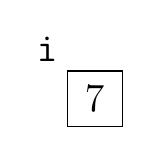
\begin{tikzpicture}
			\draw (0,0) rectangle (.7,.7);
			\draw (0,.7) node[above left]{\Large \texttt{i}};
			\draw (.35,.35) node{\Large 7};
		\end{tikzpicture}
	\end{wrapfigure}

	Une variable \texttt{i} de type primitif et contenant la valeur 7 peut se
	représenter comme ci-contre. 
	
	Il existe, en Java, 8 types primitifs~: des types primitifs numériques
	entiers, numériques à virgule flottante, les  caractères et les booléens.
	Voici ce que dit la grammaire~: 
	
	\begin{grammaire}
		\grammarrule{PrimitiveType:}
		    \grammarrule{NumericType}
		    boolean

		\grammarrule{NumericType:}
		    \grammarrule{IntegralType}
		    \grammarrule{FloatingPointType}

		\grammarrule{IntegralType:}
		    \grammarrule{(one of)}
		    byte short int long char

		\grammarrule{FloatingPointType:}
		    \grammarrule{(one of)}
		    float double
	\end{grammaire}
	
	Chaque type a une taille déterminée. 
	
	Les entiers sont codés en notation en
	complément à deux, excepté le type \pc{char} qui est un entier non-signé de
	16~bits représentant le code Unicode codé en UTF-16 du caractère
	\footnote{%	
		Pour en savoir plus sur l'Unicode, UTF8, UTF16 et UTF32, lire
		«~Unicode, UTF8, UTF16, UTF32\ldots et tutti quanti~»
		\\\url{http://namok.be/blog/?post/2009/11/30/unicode-UTF8-UTF16-UTF32-et-tutti-quanti}
	}. 
	
	Voici les tailles et les intervalles. 

	\begin{center}
		\begin{tabular}[t]{|l|>{\centering}p{1cm}|>{\centering}p{1cm}|l|}
		\hline
		\rowcolor{black!40}
		type & taille (\textit{byte})& taille (\textit{bit})	& intervalle\\
		\hline
		byte	& 1		& 8		& [-128, 127]	\\
				&		&		& [$-2^8$, $2^8-1$]	\\
		\hline
		short	& 2		& 16	& [-32\,768, 32\,767]\\
				&		&		& [$-2^{16}$, $2^{16}-1$]	\\
		\hline
		int		& 4		& 32	& [2\,147\,483\,648,2\,147\,483\,647]\\
				&		&		& [$-2^{32}$, $2^{32}-1$]	\\
		\hline
		long	& 8		& 64	& [9\,223\,372\,036\,854\,775\,808,
								9\,223\,372\,036\,854\,775\,807]\\
				&		&		& [$-2^{64}$, $2^{64}-1$]	\\
		\hline
		char	& 2		& 16	& [0,65\,535]\\
				&		&		& [0, $2^{16}-1$]	\\
		\hline
	\end{tabular}
	\end{center}

	Les nombres pseudo-réel, ou encore les nombres à virgule flottante, sont
	codés suivant la norme
	\href{https://fr.wikipedia.org/wiki/IEEE_754}{IEEE\,754}. Selon cette norme,
	un nombre est représenté avec un signe, une mantisse et un exposant. Le tout
	en base 2. Un bit est utilisé pour le signe.  

	\[
		nombre = signe~mantisse_2~2^{exposant_2} 
	\]


	\begin{center}
	\begin{tabular}[t]{|l|c|c|c|}
		\hline
		\rowcolor{black!40}
		type 	& taille (\textit{bit})	& exposant & mantisse\\
		\hline
		float	& 32					& 8		& 23\\
		\hline
		double	& 64					& 11	& 52\\
		\hline
	\end{tabular}
	\end{center}
	
	Pour les booléens, bien qu'un bit suffirait, la taille dépend 
	de l'architecture et de la \textit{jvm}. 
	
	
	
	
	\pagebreak[4]
	\subsection{Type référence}
	
	\marginicon{definition} 
	\textbf{Définition~:} 
	Une variable de type référence est une variable qui ne contient pas
	directement la valeur qui lui est assignée. Elle contient une adresse
	mémoire désignant l'endroit où est — ou sera — stockée la valeur.
	L'emplacement mémoire attribué à la variable se trouve sur la pile et a la
	même taille pour toutes les variables de type référence tandis que
	l'emplacement mémoire qui contiendra effectivement la valeur sera attribué
	sur le tas (\textit{heap}).


	\begin{wrapfigure}{r}{.3\linewidth}
		\begin{center}
		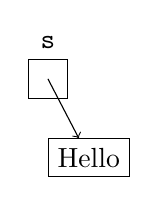
\begin{tikzpicture}
			\node[draw, minimum width=.5cm, 
				minimum height=.5cm,label={above:\texttt{s}}] (ref) {};
    		\node[draw, below of=ref, right] (string) at (0,0) {Hello};
    		\draw[->] (ref.center) -- (string);
		\end{tikzpicture}
		\end{center}
	\end{wrapfigure}
	
	\pc{String} est un type référence. 

	Une variable \texttt{s} de type référence et contenant la valeur "Hello" 
	peut se représenter comme ci-contre. 
	

	La même variable \pc{s} peut recevoir une autre valeur, par exemple beaucoup
	plus grande \pc{I would just like to say hello}. 

	\begin{java}
		String s = "Hello";
		s = "I would just like to say hello";
	\end{java}
		
	\begin{center}
		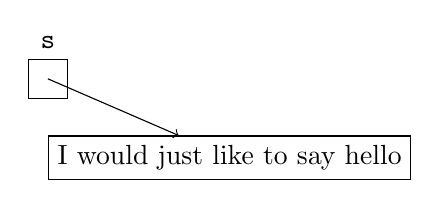
\begin{tikzpicture}
			\node[draw, minimum width=.5cm, 
				minimum height=.5cm,label={above:\texttt{s}}] (ref) {};
    		\node[draw, below of=ref, right] (string) at (0,0) {I would just like to say hello}; 
    		\draw[->] (ref.center) -- (string);
			
			%\node[draw] (ref) (0,0) rectangle (1,1);
			%\draw (0,.7) node[above of=ref, yshift=-.6cm]{\Large \texttt{s}};
			%\node[draw, below of=ref, right] (string) at (0,0) 
			%\draw[->] (ref) -- (string);
		\end{tikzpicture}
	\end{center}
	
	\paragraph{Remarque.} Même si nous ne connaissons actuellement qu'un seul
	type référence, ce seront les types les plus répandus. En effet, les types
	primitifs en Java sont au nombre de 8 comme nous l'avons vu tandis qu'il
	existe des types références prédéfinis (comme \pc{String}) et tous les types
	références définis par le développeur.  
	
	Les tableaux sont aussi des types références comme nous le verrons plus tard.
	
	
	
	\subsection{Les paramètres en Java}

	Dans nos algorithmes nous avons~: une valeur de retour, des paramètres en
	entrée et des paramètres en entrée/sortie. L'ensemble étant optionnel. Qu'en
	est-il pour le langage Java ? 

	Tout comme en algorithmique, les méthodes Java permettent de retourner une
	valeur grâce au \pc{return} \textit{Expression} de fin de méthode. Une
	méthode peut ne rien retourner. Dans ce cas, il suffit de fermer l'accolade
	ouverte en début de méthode.

	Les paramètres en Java se passent \textbf{par valeur}. En ce sens, c'est
	équivalent aux paramètres en entrée. 

	Traduisons l'exemple de la section \ref{param.entrée}
	(p.\pageref{param.entrée}) en Java. Les valeurs 3, 2 et 5 sont passées en
	argument à la méthode \pc{max3}. Les variables \pc{a}, \pc{b} et \pc{c},
	locales à la méthode \pc{max3}, reçoivent les trois valeurs. 

	\begin{java}
public class Test{
	public static void main(String[] args){
		double max;
		max = max3(3,2,5);
		System.out.println("Maximum: " + max);
	}

	public double max2(double a, double b){
		// …
	}

	public double max3(double a, double b, double c){
		double maxab;
		double max;
		maxab = max2(a,b);
		max = max2(maxab, c);
		return max;
	}
}
	\end{java}

	Il n'y a pas de paramètre en entrée/sortie en Java puisque tous les passages
	de paramètres se font par valeur. Si le paramètre est de type référence, la
	valeur que reçoit la méthode est la valeur de la référence. Même s'il n'est
	pas possible de modifier le paramètre reçu, il sera possible de modifier
	l'objet ou le tableau \textbf{référencé} par la valeur reçue en paramètre.
	En ce sens, c'est un peu un passage de paramètre en entrée/sortie. 

	
%===================
\section{Résumons}
%===================

	Reprenons tout ce que nous venons de voir avec un exemple d’algorithme qui
	possède tous les types de paramètres.

	\begin{pseudocode}[1]
		\Algo{testDivision}{}{}
			\Decl{nb1, nb2, quotient, remainder}{integers}
			\Let{nb1 \Gets 5}
			\Let{nb2 \Gets 3}
			\Let{quotient \Gets division(nb1, nb2, remainder)}
			\Write quotient
			\Write remainder
			\Let{nb1 \Gets 7}
			\Let{nb2 \Gets 9}
			\Let{quotient \Gets division(nb1, nb2, remainder)}
			\Write quotient
			\Write remainder
		\EndAlgo

		\Algo{division}{
			\Par{dividend\In}{integer}, \Par{divisor\In}{integer},\\
			\Indent\Par{remainder\In\Out}{integer}}{integer}
			\Let{\color{gray} dividend \Gets nb1} 
			\Let{\color{gray} divisor \Gets nb2} 
			\Let{\color{gray} remainder \Gets remainder} 
			\Empty
			\LComment Le code proprement dit de l’algorithme
			\Decl {quotient}{integer}
			\Let{quotient \Gets dividend DIV divisor}
			\Let{remainder \Gets dividend MOD divisor}
			\Empty
			\Let{\color{gray} remainder \Gets remainder} 
			\Return quotient
		\EndAlgo
	\end{pseudocode}
	
	Traçons-le avec~: \textit{quotient} \textbf{q}, \textit{dividend} \textbf{D}, 
	\textit{divisor} \textbf{d}, \textit{remainder} \textbf{r}.
	
	\begin{center}
	\begin{tabular}{|>{\centering\arraybackslash}m{1cm}
					|*{4}{>{\centering\arraybackslash}m{5mm}}
					|*{4}{>{\centering\arraybackslash}m{5mm}}|}
		\hline
		\rowcolor{black!50}
		  & \multicolumn{4}{c|}{\pc{testDivision}} & 
		  	\multicolumn{4}{c|}{\pc{division}} \\
		\hline
		%\# & \tiny{nb1} & \tiny{nb2} 
		%& \tiny{quotient} & \tiny{remainder}  
		%& \tiny{dividende} & \tiny{diviseur} 
		%& \tiny{remainder} & \tiny{quotient} \\
		\# & nb1 & nb2 
		& q & r  
		& D & d 
		& r & q \\
		\hline
		3  		& 5 &  &  & 	&  &  &  & \\
		4  		& {\color{gray}$\mid$}	& 3 &  &  &  &  &  &  \\
		5, 15  	& {\color{gray}$\mid$}	& {\color{gray}$\mid$} 	&  &  
				& 5 & 3  					&  &  \\
		23 		& {\color{gray}$\mid$} 	& {\color{gray}$\mid$} 	&  &  
			& {\color{gray}$\mid$}	& {\color{gray}$\mid$}	&  & 1 \\
		24 		& {\color{gray}$\mid$} 	& {\color{gray}$\mid$} 	&  &  
			& {\color{gray}$\mid$}	& {\color{gray}$\mid$}	&  2
		& {\color{gray}$\mid$} \\
		27, 5 		& {\color{gray}$\mid$} 	& {\color{gray}$\mid$} 	& 1 & 2  
		&  &  &  &  \\
		8  		& 7 & {\color{gray}$\mid$}	
		& {\color{gray}$\mid$}  &  {\color{gray}$\mid$}
		&  &  &  & \\
		9    	& {\color{gray}$\mid$}	& 9 
		& {\color{gray}$\mid$}  &  {\color{gray}$\mid$} 
		&  &  &  &  \\
		10, 15  	& {\color{gray}$\mid$}	& {\color{gray}$\mid$} 	
		& {\color{gray}$\mid$}  &  {\color{gray}$\mid$} 
			& 7  					& 9  					&  &  \\
		23 		& {\color{gray}$\mid$} 	& {\color{gray}$\mid$} 	
		  &  {\color{gray}$\mid$}  
		& {\color{gray}$\mid$}	& {\color{gray}$\mid$}	& {\color{gray}$\mid$}	&  & 0 \\
		24 		& {\color{gray}$\mid$} 	& {\color{gray}$\mid$} 	
		& {\color{gray}$\mid$}  &  {\color{gray}$\mid$}  
		& {\color{gray}$\mid$}	& {\color{gray}$\mid$}	&  7
		& {\color{gray}$\mid$} \\
		27, 10 		&{\color{gray}$\mid$} 	& {\color{gray}$\mid$} 	& 0 & 7  
		&  &  &  &  \\
		\hline
	\end{tabular}
	\end{center}

	Pour mieux se comprendre, il est utile d’introduire un peu de vocabulaire.
	
	\marginicon{definition}
	\index{paramètres formels}
	\index{paramètres effectifs}
	Les paramètres déclarés dans l’entête d’un algorithme sont appelés
	\textbf{paramètres formels}.  Les paramètres donnés à l’appel de
	l’algorithme sont appelés \textbf{paramètres effectifs}. 
	
	Les instructions en gris dans l’exemple ne sont pas écrites mais c’est comme
	si elles étaient présentes pour initialiser les paramètres formels \In{} et
	\InOut{} en début d’algorithme et pour donner des valeurs aux paramètres
	effectifs \InOut{} en fin d’algorithme.
	
	À la fin de l’algorithme, c’est comme si la valeur retournée
	\emph{remplaçait} l’appel.  Dans notre exemple, c’est donc cette valeur
	retournée qui sera affichée.
	

